%!TEX root = ../main.tex

\chapter{Sistemi Dinamici}
\label{cha:sistemi_dinamici}

Un modello matematico per descrivere le dinamiche di un sistema non lineare è quello dello \textbf{spazio degli stati}: in questo modello si pensa in termini di variabili di stato i cui valori ad un certo istante temporale sono considerati sufficienti a predire la futura evoluzione del sistema.

Sia $\vec{x}(t) = (x_1(t), \dots, x_N(t))$ il \textbf{vettore di stato} contenente le variabili di stato di un sistema dinamico non lineare, dove la variabile indipendente è il tempo $t$ e $N$ è l'ordine del sistema. È possibile descrivere un largo numero di sistemi dinamici non lineari mediante un sistema di equazioni differenziali di primo ordine chiamate \textbf{equazioni dello spazio degli stati} del tipo
\begin{displaymath}
	\frac{\dif}{\dif t} \vec{x}(t) = \vec{F}(\vec{x}(t))
\end{displaymath}
dove $\vec{F}(\vec{x})$ è una funzione che ritorna un vettore la cui $j$-esima componente è $F_j(x_j)$ con $F_j$ una qualche funzione: questo vettore prende il nome di \textbf{vettore di velocità}.

Un sistema in cui la funzione vettore $\vec{F}$ non dipende esplicitamente dal tempo è detto \textbf{autonomo}. In questo capitolo saranno trattati solo sistemi dinamici autonomi.

L'equazione dello spazio degli stati può essere vista come il descrittore del movimento di un punto nello spazio $N$-dimensionale: con lo scorrere del tempo, il punto descrive una curva nello spazio degli stati detta \textbf{traiettoria} o orbita del sistema.

La famiglia delle traiettorie, per differenti condizioni iniziali, è chiamato \textbf{ritratto degli stati} del sistema e comprende tutti i punti in cui $\vec{F}(\vec{x})$ è definita: nel caso di sistemi autonomi, per ogni punto dello spazio esiste una sola traiettoria che vi passa.

\begin{figure}[h!]
	\centering
	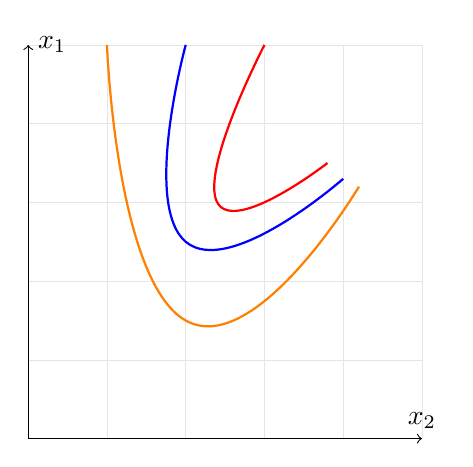
\begin{tikzpicture}
		\draw[very thin,color=gray!20] (0,0) grid (5,5);
		\draw[->] (0,0) -- (0,5) node[right] {$x_1$};
		\draw[->] (0,0) -- (5,0) node[above] {$x_2$};

		\draw[thick, color=red] plot [smooth, tension=1] coordinates{(3, 5) (2.4, 3) (3.8, 3.5)};
		\draw[thick, color=blue] plot [smooth, tension=1] coordinates{(2, 5) (2, 2.5) (4, 3.3)};
		\draw[thick, color=orange] plot [smooth, tension=1] coordinates{(1, 5) (2, 1.5) (4.2, 3.2)};
	\end{tikzpicture}
	\caption[Ritratto degli stati in un sistema dinamico]{Ritratto degli stati di un sistema dinamico di ordine $2$.}
\end{figure}

\section{Condizione di Lipschitz}
\label{sub:condizione_di_lischitz}

Affinché l'equazione dello spazio degli stati abbia soluzione e sia unica è necessario imporre alcune restrizioni su $\vec{F}(\vec{x})$: condizione sufficiente perché ci sia soluzione è che $\vec{F}(\vec{x})$ sia continua in tutti i suoi argomenti, mentre per quanto riguarda l'unicità serve una restrizione più forte, nota come \textbf{condizione di Lipschitz}.
\begin{mydef}[Condizione di Lipschitz]
	Una funzione $\vec{F}: \Omega \subseteq \mathbb{R}^n \rightarrow \mathbb{R}^m$ \emph{lipschitziana} su $\Omega$ se esiste $K \geq 0$ tale per cui 
	\begin{displaymath}
		\left \| \vec{F}(\vec{x}) - \vec{f}(\vec{y}) \right \| \le K \left \| \vec{x} - \vec{y} \right \| \qquad \forall \vec{x}, \vec{y} \in \Omega 
	\end{displaymath}
\end{mydef}
\noindent La funzione in figura~\ref{fig:lipschitz} è lipschitziana con $K=4$: se si considera un qualunque punto lungo la funzione e si tracciano le rette di coefficienti angolari $4$ e $-4$ passanti per quel punto, la funzione non sarà mai confinata tra le due rette.
\begin{figure}[h!]
	\centering
	\begin{tikzpicture}[domain=-2:2]
		\begin{axis}[restrict y to domain=-2:2, grid]
			\addplot[blue,smooth,thick] function{sin(x) * cos(4 * x)} node[above=1cm] {\tiny$\sin(x)\cos(4x)$};
			\addplot[green, thick] function{- 4 * x} node[below] {\tiny$-4x$};
			\addplot[green, thick] function{4 * x} node[above] {\tiny$4x$};
		\end{axis}
	\end{tikzpicture}
	\caption{Interpretazione grafica della Condizione di Lipschitz.}
	\label{fig:lipschitz}
\end{figure}

\section{Stati di equilibrio}
\label{sub:stabilità_degli_stati_di_equilibrio}

Un punto di equilibrio \textbf{stabile} è un punto che non risente delle piccole perturbazioni ovvero, se ci si sposta di poco da un punto stabile, il sistema continuerà a rimanere anche in futuro nelle vicinanze di quel punto. Viceversa un punto di equilibrio \textbf{instabile} è tale per cui basta una perturbazione arbitrariamente piccola dall'equilibrio per far allontanare significativamente il sistema dalla posizione iniziale.

Un vettore costante $\vec{x}$ è detto stato di equilibrio (o stazionario) se è soddisfatta la seguente condizione:
\begin{displaymath}
	\mathbf{F}(\vec{x}) = \vec{0}
\end{displaymath}
Lo stato di equilibrio è anche detto punto singolare e la traiettoria \textbf{degenera} nel punto stesso.

Si enunciano ora una serie di definizioni sulla stabilità degli stati di equilibrio.
\begin{mydef}
	Lo stato di equilibrio $\vec{x}^*$ è detto \defterm{uniformemente stabile} se, per ogni $\epsilon$ positivo, esiste $\delta$ positivo tale per cui
	\begin{displaymath}
		\|\vec{x}(0) - \vec{x}^* \| < \delta \Rightarrow \|\vec{x}(t) - \vec{x}^* \| < \epsilon \;\forall t > 0
	\end{displaymath}
\end{mydef}

\begin{mydef}
	Lo stato di equilibrio $\vec{x}^*$ è detto \defterm{convergente} se esiste $\delta$ positivo tale per cui
	\begin{displaymath}
		\|\vec{x}(0) - \vec{x}^* \| < \delta \Rightarrow \lim_{t \rightarrow \infty} \vec{x}(t) = \vec{x}^*
	\end{displaymath}
\end{mydef}

\begin{mydef}
	Lo stato di equilibrio $\vec{x}^*$ è detto \defterm{asintoticamente stabile} se è uniformemente stabile e convergente.
\end{mydef}

\begin{mydef}
	Lo stato di equilibrio $\vec{x}^*$ è detto \defterm{globalmente asintoticamente stabile} se è stabile e se tutte le traiettorie del sistema convergono a $\vec{x}^*$ per $t \rightarrow \infty$.
\end{mydef}

\section{Teorema di Lyapunov}
\label{sub:teorema_di_lyapunov}

\begin{mydef}
	La funzione $V(\vec{x})$ è \defterm{definita positiva} nello spazio degli stati $L$ se, per ogni $\vec{x} \in L$, soddisfa le seguenti proprietà:
	\begin{itemize}
		\item $V(\vec{x})$ ha derivate parziali rispetto agli elementi di $\vec{x}$ continue;
		\item $V(\vec{x}^*)=0$;
		\item $V(\vec{x})>0$ se $\vec{x} \neq \vec{x}^*$.
	\end{itemize}
\end{mydef}

\noindent Si enunciano ora i due \textbf{teoremi di Lyapunov} che forniscono condizioni sufficienti per l'esistenza di un punto stazionario.

\begin{thm}[Primo teorema di Lyapunov]
	Lo stato di equilibrio $\vec{x}^*$ è stabile se in un piccolo intorno di $\vec{x}^*$ esiste una funzione definita positiva $V(\vec{x})$ tale che la sua derivata rispetto al tempo è minore o uguale a 0 in quella regione.
\end{thm}

\begin{thm}[Secondo teorema di Lyapunov]
	Lo stato di equilibrio $\vec{x}^*$ è asintoticamente stabile se in un piccolo intorno di $\vec{x}^*$ esiste una funzione definita positiva $V(\vec{x})$ tale che la sua derivata rispetto al tempo sia strettamente minore di 0 in quella regione.
\end{thm}

\noindent Una funzione scalare $V(\vec{x})$ che soddisfa queste proprietà è detta \textbf{funzione di Lyapunov} per lo stato di equilibrio $\vec{x}^*$.

Il criterio è una generalizzazione del fatto, noto nella fisica, che un sistema meccanico, se lasciato libero di evolvere, tende a portarsi in una configurazione dove la sua energia potenziale è minima. La funzione di Lyapunov può quindi essere interpretata come una funzione di energia potenziale generalizzata. Il criterio è tuttavia una condizione sufficiente ma \textbf{non necessaria}.

Inoltre non esiste un algoritmo per trovare la funzione di Lyapunov relativa a un sistema, ma si deve cercare per tentativi, basandosi sul tipo di funzione di stato e su considerazioni puramente fisiche.